We implemented the virtual matrix elements required for
\Wbb~production in association with up to three light jets in a new
version of the \BlackHat~library \cite{Berger:2008sj}, which includes significant
upgrades for the computation of loop amplitudes with massive
particles. The library is based on the methods
presented in Chapters \ref{chap:vme2}-\ref{chap:renorm} of this
thesis. In this chapter, we provide thorough checks of the virtual
matrix elements required for \mbox{\Wbbn}~by comparing to both higher-precision targets and
automated tools. We partly showed the checks presented in this chapter
in Ref.~\cite{wbbpaper}.



\section{Numerical Stability of Virtual Matrix Elements}
\label{sec:numstab}

Previous computations with numerical unitarity have shown a good numerical stability even for high-multiplicity one-loop matrix elements (see for
example~\cite{BH:W3jDistributions,BH:W5j}). However, there exist
regions of phase space where on-shell loop-momentum parameterizations (which can e.g.~be found in \cite{Kilgore2007}) can break down. In particular, this occurs if Gram determinants\footnote{The Gram matrix is the matrix of all possible inner products of external momenta and its determinant is called the Gram determinant.}, which are found in on-shell solutions to the loop momentum, are
close to zero. This type of configuration can lead to incomplete cancellations of large contributions and
thereby induce a loss of numerical precision. 





We implemented a rescue system to control the precision of the computation, which identifies unstable
phase-space points by performing checks at several
stages of the calculation. With some minor adaptations we use the same
implementation as described in \cite{Berger:2008sj,BH:W3jDistributions}. Whenever
any of those checks fails, we switch to a higher precision computation locally
(i.e. only for the part which failed the check), using
higher-precision arithmetic as provided by the QD library \cite{QD}. The fraction of time
spent on these recomputations is normally small. Specifically, we test the vanishing of higher-rank tensor
coefficients. Tensors with rank greater than $n$, for $n$-point topologies ($n=1,2,3,4,5$) must vanish given the interactions
governed by the renormalizable QCD Lagrangian. Computing the value of an
additional higher-rank tensor coefficient comes without much extra
cost. We apply this check at the level of bubble coefficients. Through
subtractions, this captures any loss of precision in the computation
of the higher-point topologies related to the specific bubble and
allows to recompute only the numerically instable part of the
computation. Furthermore, we check
that parts of the known IR and UV divergence structure
\cite{Catani:2000ef} of a given matrix element have been reproduced correctly.
% In particular, we check that the IR double pole is an integer and
% that the UV divergence multiplied with six is also an integer. 
This assess the precision at the level of a
complete amplitude calculation. In consequence, this check demands a full recomputation in the case of failure.


We study the numerical stability of our new massive
one-loop matrix elements by comparing results computed in standard
production mode with computations fully performed in
quadruple precision~\cite{QD} (up to 32 digits of precision).




We produce distributions of the logarithmic relative error $\delta$
\begin{align}
  \delta = \log_{10}\left(\frac{|d\sigma_{V}^{\text{\texttt{prod}}} -
      d\sigma_{V}^{\text{\texttt{HP}}}|}{|d\sigma_{V}^{\text{\texttt{HP}}}|}  \right)
\end{align}
for the poles $1/\epsilon^2$, $1/\epsilon^1$ and the finite part
$\epsilon^0$, with $\epsilon$ being the dimensional regularization
parameter. The superscripts ``prod'' and ``HP'' mean standard production evaluation and
quadruple floating-point evaluation respectively. We sample over physical
phase space, as defined for the phenomenological study in the next
Chapter \ref{chap:wbb_results}, and compute for $\mathcal{O}(10^5)$
events for sample subprocesses of the most complex types in our calculations. 


%%%%%%%%%%%%% FIGURE %%%%%%%%%%%%%%%%%%
\begin{figure}[tbh]
\begin{center}
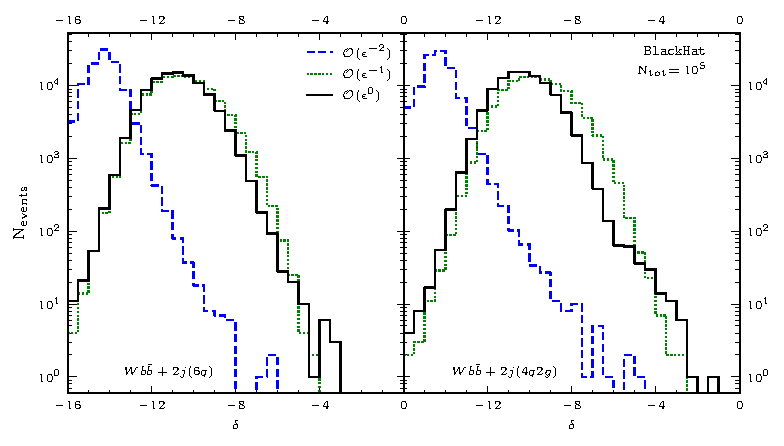
\includegraphics[clip,scale=1.2]{plots/numstab2j}
\end{center}
\caption{Relative logarithmic error distributions of full-color
  matrix elements for two types of subprocesses contributing to
  \Wbbnj[2]~production, that is $0\rightarrow Wb{\bar b}q{\bar q}'Q{\bar
    Q}$ (left) and $0\rightarrow Wb{\bar b}q{\bar q}'gg$ (right). We use a set of $10^5$
phase-space points sampled for the LHC with $\sqrt{s}=13$ TeV in the same way as the phenomenological
study presented in Chapter \ref{chap:wbb_results}. We use a dedicated calculation in
quadruple precision for computing target results to compare against. The dashed (blue) line represents the precision of the double pole, the dotted
(green) line represents the single pole and the
solid (black) line the precision of the finite piece of the calculation.}
\label{fig:numstab2j}
\end{figure}
%%%%%%%%%%%%%%%%%%%%%%%%%%%%%%%%%%%%%%%

In Fig.~\ref{fig:numstab2j} and Fig.~\ref{fig:numstab3j}, we show
results for \Wbbnj[2]~and \Wbbnj[3]~production, respectively. We include the
two types of
subprocesses for \Wbbnj[2] : those with four quarks and two gluons (associated by crossing two
partons into the final state to the process $0\rightarrow Wb{\bar b}q{\bar q}'gg$),
and those with six quarks ($0\rightarrow Wb{\bar b}q{\bar q}'Q{\bar Q}$).
For \Wbbnj[3]{} we show the cases with four quarks and three gluons
($0\rightarrow Wb{\bar b}q{\bar q}'ggg$),
and with six quarks and one gluon ($0\rightarrow Wb{\bar b}q{\bar q}'Q{\bar Q}g$).
%
Each figure shows the estimated precision of the computation of the double and
single pole as well as the finite piece for each amplitude. The double pole is
commonly computed with an accuracy of 14 digits, while the single pole and the
finite piece distributions peak at about 10 digits.


%%%%%%%%%%%%% FIGURE %%%%%%%%%%%%%%%%%%
\begin{figure}[tbh]
\begin{center}
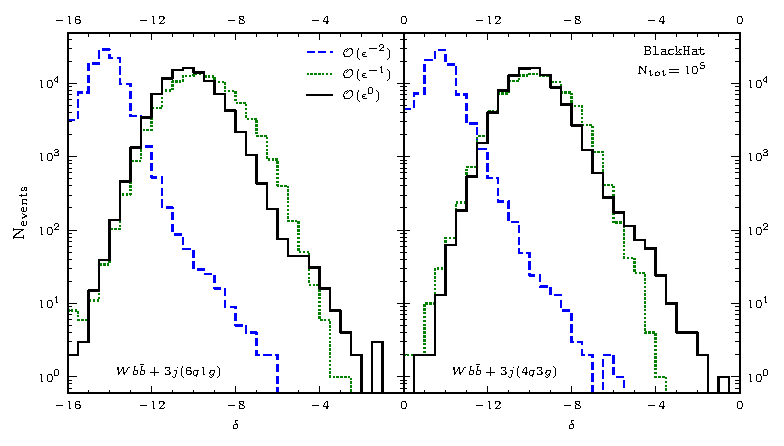
\includegraphics[clip,scale=1.2]{plots/numstab3j}
\end{center}
\caption{As in Fig.~\ref{fig:numstab2j} but for \Wbbnj[3]{}
  production. This time, we consider only leading-color contributions to the one-loop matrix elements.
    To the left we show subprocesses associated to $0\rightarrow Wb{\bar
b}q{\bar q}'Q{\bar Q}g$, and on the right the ones associated to
    $0\rightarrow Wb{\bar b}q{\bar q}'ggg$ .}
\label{fig:numstab3j}
\end{figure}
%%%%%%%%%%%%%%%%%%%%%%%%%%%%%%%%%%%%%%%


Overall, our computation has a very good precision, with less than $1$ in $10^4$ phase-space
points computed to an accuracy worse than three digits.
%
We attribute some of the few points in the low-precision tail to the
fact that the scale set by the bottom mass $m_b$ and other scales of
the problem $s_{ij}$ at sufficiently high energy are separated by several orders of magnitude.
The ratios of the form $(m_b^2/s_{ij})^k$ enter loop-momentum
parameterizations and can cause loss of precision. However, we have observed that
the contribution of the points in the low-precision tail is significantly smaller than the total statistical errors for the observables studied.



\section{Phase-Space Point Comparison Against Automated Tools}
\label{sec:pspcomp}
We carried out a number of checks with the new implementation of \BlackHat{}. %version
%\vBH{}. 
We systematically reproduced matrix elements that were implemented in the earlier versions of the library such as those for $V$+jets, jets and $VV$+jets production ($V=W,Z$) and found
excellent agreement. Furthermore, the explicit cancellation of infrared poles of renormalized one-loop matrix
elements is checked by comparing to the integrated subtraction terms as performed with the~\SHERPA{} library.

We reproduced the results for primitive amplitudes including a top-quark pair and three gluons as presented by Ellis \textit{et al.}
in~\cite{Ellis:2008ir}. Even more, we cross checked fully interfered, matrix-element squared results against
automated tools available on the market. In particular, this includes comparisons of all
one-loop matrix elements necessary for $pp\rightarrow t\bar t+(\leq 2)-$jet and
$pp\rightarrow b\bar b+(\leq 2)-$jet at NLO QCD with the
\texttt{RECOLA}~\cite{Actis:2016mpe} and
\texttt{OpenLoops}~\cite{Cascioli:2011va} libraries (both powered by the
\texttt{Collier} library~\cite{Denner:2016kdg}), as well as all the ones needed
for $Wb\bar b+(\leq3)-$jet with \texttt{RECOLA}.

%%%%%%%%%%%%%%%%%%%%%%%%%%%%%%%%%%%%%%%%
%%%%%%%%%%%%%%%%%%%%%%%%%%%%%%%%%%%%%%%%
%Table Acc comparison
\begin{table}[]
\centering
\begin{tabular}{cllll}
  \hline\hline
  \noalign{\vskip 2mm}
  & Process & $\Delta_{V,\epsilon^{-2}}$  &
  $\Delta_{V,\epsilon^{-1}}$ &
  $\Delta_{V,\epsilon^0}$ \\ 
  \noalign{\vskip 2mm}
  \hline
  \noalign{\vskip 1mm}
  \multicolumn{1}{c}{ \multirow{2}{*}{$n=0$}}& $u \bar{d} \rightarrow e^+ \bar{\nu}_e b\bar{b}$ & $9.508\cdot 10^{-14}$
 &$5.925 \cdot 10^{-13}$  &$3.338\cdot 10^{-12}$  \\
  \multicolumn{1}{c}{}&$d \bar{u} \rightarrow e^- \nu_e b\bar{b}$ & $9.989\cdot 10^{-14}$ &
 $6.602 \cdot 10^{-13}$ & $3.507 \cdot 10^{-12}$ \\
 \noalign{\vskip 1mm}
 \hline
 \noalign{\vskip 1mm}
 \multicolumn{1}{c}{\multirow{2}{*}{$n=1$}}& $u \bar{d} \rightarrow e^+ \bar{\nu}_e b\bar{b} g$ &$6.577\cdot
 10^{-13}$  & $4.114\cdot 10^{-11}$  & $5.329\cdot 10^{-10}$ \\
 \multicolumn{1}{c}{}& $d \bar{u} \rightarrow e^- \nu_e b\bar{b}g$
 &$7.224\cdot 10^{-13}$  & $4.515\cdot 10^{-11}$ & $6.012\cdot
 10^{-10}$ \\
 \noalign{\vskip 1mm}
 \hline
 \noalign{\vskip 1mm}
 \multicolumn{1}{c}{ \multirow{6}{*}{$n=2$}}& $u \bar{d} \rightarrow e^+ \bar{\nu}_e b\bar{b} d \bar{d}$&
  $4.709\cdot 10^{-12}$  &  $2.711\cdot 10^{-10}$ &  $3.217\cdot 10^{-9}$  \\
 \multicolumn{1}{c}{} & $u \bar{d} \rightarrow e^+ \bar{\nu}_e b\bar{b} s\bar{s} $&   $5.351\cdot 10^{-12}$  &  $2.185\cdot 10^{-10}$ &  $3.100\cdot 10^{-9}$  \\
 \multicolumn{1}{c}{} & $u \bar{d} \rightarrow e^+ \bar{\nu}_e b\bar{b} g g$&  $1.036\cdot
 10^{-11}$  &  $7.192\cdot 10^{-10}$ &  $1.007\cdot 10^{-8}$ \\
 \multicolumn{1}{c}{} & $d \bar{u} \rightarrow e^- \nu_e b\bar{b} d \bar{d}$ &$5.300\cdot 10^{-12}$  & $2.524\cdot 10^{-10}$ & $2.774\cdot 10^{-9}$\\
 \multicolumn{1}{c}{} & $d \bar{u} \rightarrow e^- \nu_e b\bar{b}s\bar{s}$ &$5.260\cdot 10^{-12}$  & $1.965\cdot 10^{-10}$ & $2.773\cdot 10^{-9}$\\
 \multicolumn{1}{c}{} & $d \bar{u} \rightarrow e^- \nu_e b\bar{b}gg$
 &$9.867\cdot 10^{-12}$  & $6.525\cdot 10^{-10}$ & $8.646\cdot
 10^{-9}$\\
 \noalign{\vskip 1mm}
 \hline
 \noalign{\vskip 1mm}
  \multicolumn{1}{c}{ \multirow{4}{*}{$n=3$}}&$u \bar{d} \rightarrow e^+ \bar{\nu}_e b\bar{b} d \bar{d} g$   &$6.412\cdot 10^{-11}$  & $2.211\cdot 10^{-9}$ & $7.703\cdot 10^{-8}$ \\
 \multicolumn{1}{c}{}&$u \bar{d} \rightarrow e^+ \bar{\nu}_e b\bar{b} g g g$ &$1.347\cdot 10^{-10}$  & $3.023\cdot 10^{-9}$ & $2.762\cdot 10^{-7}$ \\
 \multicolumn{1}{c}{} & $d \bar{u} \rightarrow e^- \nu_e b\bar{b} d \bar{d} g $ &$6.571\cdot 10^{-11}$  & $2.077\cdot 10^{-9}$ & $7.432\cdot 10^{-8}$\\ 
 \multicolumn{1}{c}{} & $d \bar{u} \rightarrow e^- \nu_e b\bar{b} g g
 g $  &$1.530\cdot 10^{-10}$  & $3.031\cdot 10^{-9}$ & $2.783\cdot
 10^{-7}$\\ 
 \noalign{\vskip 1mm}
 \hline\hline
\end{tabular}
\caption{The logarithmically averaged relative deviation of poles in
  $\epsilon$ as well as the finite part of virtual matrix
  elements computed with \BlackHat{} and \recola. We averaged over 1000 randomly
  chosen phase-space points. Shown are the deviations for exemplary
  subprocesses contributing to \Wbbn .}
\label{tab:reldev}
\end{table}

%%%%%%%%%%%%%%%%%%%%%%%%%%%%%%%%%%%%%%%%
%%%%%%%%%%%%%%%%%%%%%%%%%%%%%%%%%%%%%%%%


For the latter comparison of virtual matrix elements required for $Wb\bar
b+(\leq3)-$jet with \texttt{RECOLA}, we compute the logarithmically averaged
relative deviation
\begin{align}
\log_{10}\Delta_{V}=\frac{1}{N_{tot}} \sum_{j=1}^{N_{tot}} \log_{10}
  \left( \frac{|d\sigma_{V, \text{\BlackHat{}}}^{j} - d\sigma_{V,
        \text{\recola}}^{j}|}{|d\sigma_{V,\text{\recola}}^j|} \right)
\end{align}
where $N_{tot}$ denotes the total number of phase space points
considered. We compare for exemplary subprocesses contributing to
\Wbbn~and sample over 1000 randomly chosen phase-space points for
each of the subprocesses considered. In Table \ref{tab:reldev}, we show $\Delta_{V}$ for both singe pole
$1/\epsilon^2$ and double pole $1/\epsilon^1$ as well as the finite part $\epsilon^0$.


Overall we find good agreement for all subprocesses considered between the
results computed with \recola~and \BlackHat{}. The average relative deviation increases
with the multiplicity of light jets $n$ since more particles in the final
state lead to an increased complexity due to more contributions to the calculation. Also the presence of external
gluons makes the agreement worse. The average relative
deviation for the case $n=0$ lies around $\mathcal{O}(10^{-14})$ for the double pole,
$\mathcal{O}(10^{-13})$ for the single pole and
$\mathcal{O}(10^{-12})$ for the finite term,
corresponding to an agreement of $12$ digits on average. For the
highest multiplicity case $n=3$, it decreases to around $\mathcal{O}(10^{-10})$ for the double pole,
$\mathcal{O}(10^{-9})$ for the single pole and
$\mathcal{O}(10^{-7})$ for the finite term,
corresponding to an agreement of $7$ digits on average. Whereas we have good control over the precision of our calculation with \BlackHat{}, see previous Sec.~\ref{sec:numstab}, no corresponding precision data for \recola{} is publicly available. A similar comparison against
\OL~\cite{Cascioli:2011va} for the lower
multiplicity cases $n\leq 2$ shows a comparable agreement.


\section{Validation of Integrated Total Cross Sections}
We complete the validation of our new matrix elements by dedicated comparisons at the level of physical observables
against the \texttt{MCFM} program~\cite{mcfm7} for the inclusive production of \Wbb{}
at NLO QCD at the LHC with $\sqrt{s}=13$ TeV. We find agreement at the
permil level for both total cross sections and differential
distributions. The matrix-elements
implemented in \texttt{MCFM} were first reported
in \cite{Badger:2010mg}, where analytic expressions for the QCD NLO
corrections for \Wbb~including decay correlations and a non-zero
bottom mass were found.


For our comparison, we use the renormalization and
factorization scale \murf[M_W]. We use the 5-flavor \texttt{MSTW2008} LO (\texttt{MSTW2008lo}) and NLO (\texttt{MSTW2008nlo})
PDFs~\cite{MSTW08} interfaced through LHADPF 6.1.3 \cite{LHAPDF} at the respective orders with $\alpha_s(M_Z) = 0.133551$ (LO) and $\alpha_s(M_Z) = 0.114904$ (NLO).


We use real values for the electroweak
parameters as specified in Tab.~\ref{tab:ewinput}. However, for this
comparison we use a non-diagonal CKM
matrix in the Wolfenstein parameterization \cite{WoCKM} with the
parameter $\lambda=0.2272$.  All light quarks ($u$, $d$, $s$, $c$) are treated as massless and
bottom quarks are treated massive if they appear in the final
state. The mass of the bottom quark is set according to the PDF to
$m_b=4.75$ GeV. We do include contributions from closed top quark loops, with the top mass
set to $m_t=173.5$ GeV. Bottom quarks in virtual closed loops are
treated as massless particles in accordance with the scheme implemented in MCFM.

We reconstruct b-jets by using the \texttt{anti-$k_T$} algorithm
\cite{antikT} as implemented in the package \texttt{Fastjet}
\cite{Cacciari:2005hq,Cacciari:2011ma}, with jet-radius parameter $R=0.5$. We require
the b-jets to have a minimum transverse-momentum of $p_T>25$ GeV.

We integrated three statistically independent samples. The
total integrated cross section in pb for both \Wbbm~and \Wbbp~are shown in Table
\ref{tab:xsmcfmWmbb}. The values in parenthesis next to the central value denote the uncertainty
associated to the numerical integration. The results obtained by
\texttt{MCFM} and \BlackHat\texttt{+}\SHERPA{}~are integrated to about $0.1\%$. 

%We also show the mean and its standard error in Fig.~\ref{fig:mcfm_bh}. Doing an independent two-sample \textit{t}-test, we find that the two-tailed p-value is given for \Wbbm~by $p=0.97$ (LO) and $p=0.039$ (NLO) and for \Wbbp~by $p=0.75$ (LO) and $p=0.064$ (NLO), thus both NLO \textit{p}-values lie close to a significance level of $5\%$. In light of the small absolute value of the differences and taking the quoted Monte Carlo errors with a grain of salt, we do not obtain a larger sample set. 

%%%%%%%%%%% TABLE xs mcfm bh Wm  %%%%%%%%%%%%%%%%%%%%%%%%%%
\begin{table}[ht]
  \begin{centering}
  \begin{tabular}{ccccccc}
    \hline\hline
    \noalign{\vskip 2mm}
    Run  & \Wbbm~LO &   \Wbbm~NLO &$K$-factor &\Wbbp~LO &   \Wbbp~NLO
    & $K$-factor \\
    \noalign{\vskip 2mm}
    \hline
    \noalign{\vskip 2mm}
    \texttt{MCFM 1}  & $1.0961(7)$ & $2.3613(23)$   &$2.154$ &$1.7644(11)$ &$3.6788(37)$ & $2.085$ \\
    \texttt{MCFM 2}  & $1.0972(8)$ & $2.3542(21)$   &$2.146$ &$1.7644(12)$ &$3.6790(42)$ & $2.085$ \\
    \texttt{MCFM 3}  & $1.0968(7)$ & $2.3562(39)$   &$2.148$
    &$1.7655(11)$ &$3.6766(34)$ & $2.082$  \\
    \noalign{\vskip 2mm}
    \hline
    \noalign{\vskip 2mm}
    \texttt{BlackHat 1}& $1.0973(3)$ & $2.3618(25)$  & $2.152$& $1.7652(6)$   &$3.6877(48)$ & $2.089$\\
    \texttt{BlackHat 2}& $1.0962(5)$ & $2.3596(30)$  & $2.153$& $1.7643(9)$   &$3.6804(56)$ & $2.086$\\
    \texttt{BlackHat 3}& $1.0966(5)$ & $2.3649(36)$  & $2.157$& $1.7640(8)$   &$3.6809(40)$ & $2.087$\\
    \noalign{\vskip 2mm}    
    \hline\hline
  \end{tabular}
  \caption{Total integrated cross-section at LO and NLO for
    \Wbbm~production (left) and \Wbbp~production (right) in
    \textit{pb} as well as the ratio of the NLO to LO result ($K$-factor). Shown are the results of three
    statistically independent runs of \texttt{MCFM} and \BlackHat\texttt{+}\SHERPA. The uncertainty
    associated to the numerical integration is given in parenthesis
    next to the central value.}
  \label{tab:xsmcfmWmbb}
\end{centering}
\end{table}
%%%%%%%%%%%%%%%%%%%%%%%%%%%%%%%%%%%%%%%

The results agree to the expected level, in particular
in light of the small absolute difference of the
cross-sections. The agreement after numerical
integration validates the setup of \BlackHat\texttt{+}\SHERPA{} against MCFM.

